% Star tracker-accelerometro-gps
Esistono diversi tipi di sensori per la determinazione dell'assetto e
dell'orbita del satellite.
\begin{itemize}
\item Sensori inerziali: come accelerometri o giroscopi, sensibili alla causa
del movimento
\item Sensori d'assetto: come i magnetometri, gli star trackers o i GPS,
osservano il moto
\item Sensori di posizione: come i GPS, individuano la posizione dello strumento
\end{itemize}
Verranno descritti solo i sensori utilizzati ai fini della simulazione.
\paragraph{Accelerometro}
Esso permette di misurare l'accelerazione lineare del centro di massa.
L'implemetazione è realizzata mediante una piccola massa (proof-mass)
all'interno di una scatola, che la protegge dalle
forze esterne cui è soggetto il satellite. Per fare ciò, è necessario che il
satellite insegua la massa, o che la massa insegua il satellite. La proof-mass
è soggetta alla sola forza gravitazionale, quindi è in caduta libera,
ciò implica che la forza utilizzata per mantenere la massa di prova ferma
rispetto alla scatola che la contiene, può essere utilizzata per misurare le
forze esterne al satellite, vedi figura \ref{fig:accelerometro} 
\begin{figure}[htp]
\begin{center}
  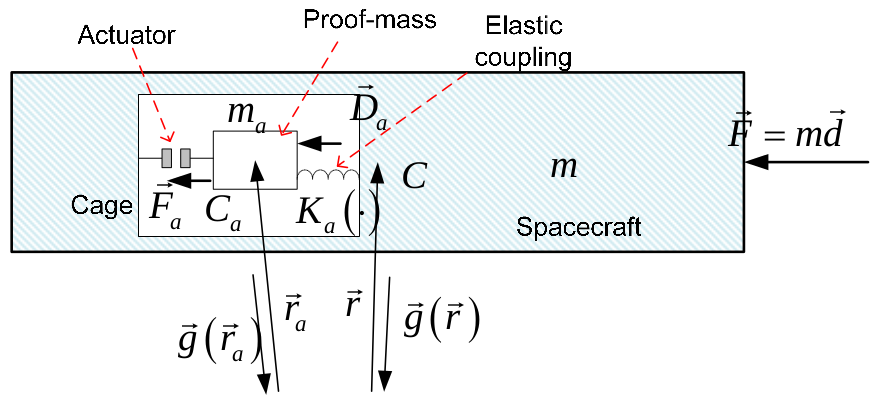
\includegraphics[width=\textwidth]{modelling/attitude_kinematics_and_dynamics/image/accelerometro.png}
  \caption{Massa di prova di un accelerometro}
  \label{fig:accelerometro}
\end{center}
\end{figure}
Indichiamo con $m$ la massa del satellite e con $m_a$ la massa della proof-mass,
$\vec{r}$ e $\vec{v}$ indicano la posizione  e la velocità del satellite, mentre
$\vec{r}_a$ e $\vec{v}_a$ indicano la posizione e la velocità della massa di
prova. Le equazioni di Newton della massa $m_a$ e del satellite sono
\begin{equation}
\dot{\vec{v}}(t)=-\vec{g}(\vec{r}(t))+\frac{\vec{F}(t)-\vec{F}_a(t)}{m}
\end{equation}
\begin{equation}
\dot{\vec{v}}_a(t)=-\vec{g}(\vec{r}_a(t))+\frac{\vec{F}_a(t)}{m_a}+\frac{\vec{D}_a(t)}{m_a}
\end{equation}
dove $\vec{D}_a$ indica le forze parassite agenti sulla proof-mass. Attraverso
la misura di $\vec{F}_a$ è quindi possibile risalire alle forze esterne al
satellite.

Tra gli errori di misura che affliggono le misurazioni effettuate tramite un accelerometro
è presente il bias, cioè un offset sistematico, dovuto alla tecnologia costruttiva, che viene
aggiunto alle misure. Nel controllo, purtroppo, tale errore viene interpretato come disturbo
dall’osservatore che quindi stima il drag sommato alla polarizzazione dell’accelerometro. Per
ovviare a tale difetto si agisce eliminando il valor medio del bias dall’uscita dell’osservatore.
Tuttavia l’orbita non sarà mai priva di accelerazioni non gravitazionali, poiché tra gli errori
dell’accelerometro è presente anche una deriva aleatoria.
Nel simulatore l'accelerometro è utilizzato per effettuare il controllo
drag-free, ovvero per eliminare i disturbi dovuti all'interazione con le
molecole dell'atmosfera.
\paragraph{Star tracker}
Sfrutta l'individuazione delle stelle fisse, tramite un sensore ottico, per poi
confrontare ciò che vede con un catalogo stellare e, attarverso degli algoritmi,
ricavare una posizione. L'onda elettromagnetica, emessa dalla stella osservata,
viene rilevata sul sensore come un piano, date le enormi dimensioni.
Un sensore CCD, tramite un obbiettivo, incanala l'onda sul piano immagine,
facendo arrivare la rappresentazione della stella come un punto sul piano (focalizzazione). Il punto
sul piano immagine viene rappresentato attraverso una delta di Dirac, per
poterne esprimere l'intensità, misurata dalla magnitudine (in scala
logaritmica).
Il vettore coordinate ${\bf v_k}$ della stella è dato nel sistema inerziale
J2000, in funzione dell'ascensione retta $\alpha_k$ e della declinazione
$\delta_k$
\[ {\bf v_k}=\begin{bmatrix}
\cos\alpha_k\cos\delta_k \\
\sin\alpha_k\cos\delta_k \\
\sin\delta_k
\end{bmatrix} \]
Il generico vettore ${\bf v_s}$ delle coordinate della stella visualizzata è
dato nel sistema di riferimento dello strumento
$\mathfrak{R}_s=\{O_s,\bar{i}_s,\bar{j}_s,\bar{k}_s\}$ dove l'ultimo asse è
quello ottico. ${\bf v_s}$ si ottiene facendo ruotare l'asse ottico $\bar{k}_s$
attorno $\bar{j}_s$ di un angolo $\theta_s$ e successivamente attorno l'asse
$\bar{i}_s$ di un angolo $\phi_s$
\[
{\bf v_s}=X(-\phi_s)Y(-\theta_s)\begin{bmatrix} 0 \\ 0 \\ 1 \end{bmatrix} =
\begin{bmatrix}
1 & 0 & 0 \\
0 & \cos\phi_s & -\sin\phi_s \\
0 & \sin\phi_s & \cos\phi_s
\end{bmatrix}
\begin{bmatrix}
\sin\theta_s \\ 0 \\ \cos\theta_s
\end{bmatrix} =
\begin{bmatrix}
\sin\theta_s \\
-\sin\phi_s\cos\theta_s \\
\cos\phi_s\cos\theta_s
\end{bmatrix}
\]
Il field of view (FOV), ovvero il campo di visuale, è definito dal più ampio
angolo che riesce a catturare l'immagine
\[
FOV:|\theta_s|\leq\theta_{s_{max}}/2, \ |\phi_s|\leq\phi_{s_{max}}/2, \
\theta_{s_{max}}=\phi_{s_{max}}
\]
\paragraph{GPS}
Il Global Positioning System è un sistema di misura della posizione assoluta. Il
principio di funzionamento si basa su un metodo di posizionamento sferico
(trilaterazione), che parte dalla misurazione del tempo impiegato da un segnale
radio a percorrere la distanza satellite-ricevitore.
Poiché il ricevitore non conosce quando è stato trasmesso il segnale dal
satellite, per il calcolo della differenza dei tempi il segnale inviato dal
satellite è di tipo orario, grazie all'orologio atomico presente sul satellite:
il ricevitore calcola l'esatta distanza di propagazione dal satellite a partire
dalla differenza (dell'ordine dei microsecondi) tra l'orario pervenuto e quello
del proprio orologio sincronizzato con quello a bordo del satellite, tenendo
conto della velocità di propagazione del segnale.
Nel simulatore è possibile utilizzare il GPS, perché il satellite in questione
si trova in un'orbita relativamente bassa ed è quindi possibile ricevere
segnali dai satelliti in orbite più alte, il GPS viene, quindi utilizzato per
ricostruire l'assetto del satellite e la sua posizione.

